%%%%%%%%%%%%%%%%%%%%%%%%%%%%%%%%%%%%%%%%%%%%%%%%%%%%%%%%%%%%%%%%%%%%%%%%%%%%%%%%
% Preámbulo                                                                    %
%%%%%%%%%%%%%%%%%%%%%%%%%%%%%%%%%%%%%%%%%%%%%%%%%%%%%%%%%%%%%%%%%%%%%%%%%%%%%%%%

\documentclass[11pt,a4paper,titlepage,twoside,openright,openbib]{report}

%%% RELACIÓN DE VARIABLES A PERSONALIZAR %%%
%\def\lingua{gal}
\def\lingua{esp} % descomenta esta liña se redactarás a memoria en español
%\def\lingua{eng} % descomenta esta liña se redactarás a memoria en inglés
\def\nome{Diego Trabazo Sardón}                             % substitúe aquí o teu nome
\def\nomedirectorA{José Carlos Dafonte Vázquez}             % substitúe aquí o nome de quen dirixe
\def\titulo{Sistema para la extracción automática de información estructurada a partir de documentos con
elementos de maquetación comunes} % substitúe aquí o título do teu TFG
%\def\mencion{NOME DA MENCIÓN}                        % descomenta a mención correspondente
\def\mencion{COMPUTACIÓN}
%\def\mencion{ENXEÑARÍA DO SOFTWARE}
%\def\mencion{ENXEÑARÍA DE COMPUTADORES}
%\def\mencion{SISTEMAS DE INFORMACIÓN}
%\def\mencion{TECNOLOXÍAS DA INFORMACIÓN}

\def\renomearcadros{si} % descomenta esta liña se redactas a memoria en español e prefires que
                         % os "cuadros" e o "índice de cuadros" se renomeen
                         % a "tablas" e "índice de tablas" respectivamente

\usepackage{estilo_tfg}

% Cambia el tipo y tamaño de la fuente monoespaciada en todo el documento
\setmonofont[Scale=MatchLowercase]{IBMPlexMono}

% Lista de paquetes potencialmente interesantes (uso baixo demanda)

% \usepackage{alltt}       % proporciona o entorno alltt, semellante a verbatim pero que respecta comandos
% \usepackage{enumitem}    % permite personalizar os entornos de lista
% \usepackage{eurofont}    % proporciona o comando \euro
% \usepackage{float}       % permite máis opcións para controlar obxectos flotantes (táboas, figuras)
% \usepackage{hhline}      % permie personalizar as liñas horizontais en arrays e táboas
% \usepackage{longtable}   % permite construir táboas que ocupan máis dunha páxina
% \usepackage{lscape}      % permite colocar partes do documento en orientación apaisada
% \usepackage{moreverb}    % permite personalizar o entorno verbatim
% \usepackage{multirow}    % permite crear celdas que ocupan varias filas da mesma táboa
% \usepackage{pdfpages}    % permite insertar ficheiros en PDF no documento
% \usepackage{rotating}    % permite diferentes tipos de rotacións para figuras e táboas
% \usepackage{subcaption}  % permite a inclusión de varias subfiguras nunha figura
% \usepackage{tabu}        % permite táboas flexibles
% \usepackage{tabularx}    % permite táboas con columnas de anchura determinada
\usepackage{minted} % proporciona código coloreado para el código


%%%%%%%%%%%%%%%%%%%%%%%%%%%%%%%%%%%%%%%%%%%%%%%%%%%%%%%%%%%%%%%%%%%%%%%%%%%%%%%%
% Corpo                                                                        %
%%%%%%%%%%%%%%%%%%%%%%%%%%%%%%%%%%%%%%%%%%%%%%%%%%%%%%%%%%%%%%%%%%%%%%%%%%%%%%%%

\begin{document}

 %%%%%%%%%%%%%%%%%%%%%%%%%%%%%%%%%%%%%%%%
 % Preliminares do documento            %
 %%%%%%%%%%%%%%%%%%%%%%%%%%%%%%%%%%%%%%%%

 \begin{titlepage}
  
  \hspace*{128pt}
  \textcolor{udcpink}{{\fontencoding{T1}\fontfamily{phv}\selectfont Facultade de Informática}}\\[-32pt]

  \begin{center}
    
\includegraphics[scale=0.3]{imaxes/udc}\\[35pt]

    {\large TRABALLO FIN DE GRAO \\
            GRAO EN ENXEÑARÍA INFORMÁTICA \\
            MENCIÓN EN \mencion } \\[100pt]
    
    \begin{huge}
      \begin{spacing}{1.3}
        \bfseries \titulo
      \end{spacing}
    \end{huge}
  \end{center}
  
  \vfill
  
  \begin{flushright}
    {\large
    \begin{tabular}{ll}
      {\bf Estudante:} & \nome \\
      {\bf Dirección:} & \nomedirectora1 \\ % COPIA E PEGA ESTA LIÑA SE O PRECISAS
    \end{tabular}}
  \end{flushright}
  \rightline{A Coruña, \datasimple\today.}
\end{titlepage}

 \paxinaenbranco
 \dedicatoria{Dedicatoria} % escribe neste comando o teu texto de dedicatoria
 \paxinaenbranco
 \paxinaenbranco
 \begin{agradecementos}
 \blindtext                % substitúe este comando polo teu texto de agradecementos
 \end{agradecementos}
 \paxinaenbranco
 %%%%%%%%%%%%%%%%%%%%%%%%%%%%%%%%%%%%%%%%%%%%%%%%%%%%%%%%%%%%%%%%%%%%%%%%%%%%%%%%

\begin{abstract}\thispagestyle{empty}

Este TFG tiene por objetivo la creación de una solución de entorno servidor, para automatizar la adquisición de información desde fuentes de datos semiestructuradas, como son los PDF. El proyecto se enmarca en el ámbito de la transición de organizaciones, públicas o privadas, hacia la informatización de los procesos.
Se centra específicamente en documentos donde existe un modelo común de maquetación, que los representan. Tanto si los ficheros PDF han sido creados digitalmente, por ejemplo, por un sistema de facturación, como si son simplemente producidos a partir de imágenes obtenidas por un escáner, desde documentos en papel, no resulta trivial recuperar de forma eficaz, la información contenida en ellos. El sistema realiza la extracción de la información, construye una representación interna de la misma gracias a sus coordenadas físicas, y posteriormente, la transforma a un formato estructurado, por medio de técnicas de procesamiento de lenguajes formales, en particular mediante los analizadores Flex y GNU Bison.

  \vspace*{25pt}
  \begin{segundoresumo}
This Bachelor's Degree Final Project aims to create a backend solution for automating information acquisition from semi-structured sources, like PDF file format. The project is framed within the scope of easing the transition of public or private organizations towards more process informatization.
It is specifically centered in the case of documents where there is a common layout that represents them. Whether the PDF files were digitally created, for example, by a billing system or they are simply sourced from images produced by a scanner, from paper documents, it is not trivial to effectively get back the information they hold. The system performs the information extraction, builds an internal representation thanks to the data's physical coordinates and finally, transforms that representation to an structured format, by employing formal languages processing techniques, particularly leaning on Flex and GNU Bison anylizers.
  \end{segundoresumo}

\newpage
\vspace*{25pt}
\begin{multicols}{2}
\begin{description}
\item [\palabraschaveprincipal:] \mbox{} \\[-20pt]
  \begin{itemize}
      \item Oficina sin papel 
      \item Lenguajes formales
      \item Flex
      \item Bison
      \item Transformada de Hough
      \item Procesamiento de Lenguajes
  \end{itemize}
%  \blindlist{itemize}[7] % substitúe este comando por un itemize
                         % que relacione as palabras chave
                         % que mellor identifiquen o teu TFG
                         % no idioma principal da memoria (tipicamente: galego)
\end{description}
\begin{description}
\item [\palabraschavesecundaria:] \mbox{} \\[-20pt]
  \begin{itemize}
      \item Paperless Office
      \item Formal languages
      \item Flex
      \item Bison
      \item Hough Transform
  \end{itemize}

  %\blindlist{itemize}[7] % substitúe este comando por un itemize
                         % que relacione as palabras chave
                         % que mellor identifiquen o teu TFG
                         % no idioma secundario da memoria (tipicamente: inglés)
\end{description}
\end{multicols}

\end{abstract}

%%%%%%%%%%%%%%%%%%%%%%%%%%%%%%%%%%%%%%%%%%%%%%%%%%%%%%%%%%%%%%%%%%%%%%%%%%%%%%%%

 \paxinaenbranco

 \pagenumbering{roman}
 \setcounter{page}{1}
 \bstctlcite{IEEEexample:BSTcontrol}

 \tableofcontents
 \listoffigures
 \listoftables
 \cleardoublepage
 
 \pagenumbering{arabic}
 \setcounter{page}{1}

 %%%%%%%%%%%%%%%%%%%%%%%%%%%%%%%%%%%%%%%%
 % Capítulos                            %
 %%%%%%%%%%%%%%%%%%%%%%%%%%%%%%%%%%%%%%%%

 %\chapter{Introdución}
\label{chap:introducion}

\lettrine{P}{rimer} capítulo da memoria, onde xeralmente se exporán as
liñas mestras do traballo, os obxectivos, etc. Incluimos un par de
exemplos de citas~\cite{ErlangBook,ErlangWebBook} e de referencias
internas (sección \ref{sec:mostra}, páxina \pageref{sec:mostra}).

\Blindtext

\section{Sección de mostra}
\label{sec:mostra}

\Blindtext

\subsection{Subsección de mostra}

\Blindtext

 %\chapter{Contido demostrativo}
\label{chap:demo}

\lettrine{E}{ntre} a introdución e as conclusións, o documento conterá
tantos capítulos como sexa preciso, sempre con coidado de non rebasar
o límite de 80 páxinas fixado polo regulamento de TFGs.

Empregaremos éste de xeito demostrativo, para ilustrar o uso de
elementos habituais que poidan ser de utilidade.

\section{Inclusión de imaxes}

Se precisamos imaxes no noso documento, incluirémolas do xeito que se
indica na figura~\ref{fig:exemplo} (páxina~\pageref{fig:exemplo}). Se
o facemos así, \LaTeX ubicará cada imaxe no mellor lugar posible,
lugar que pode variar a medida que o documento vaia crecendo coa
inclusión de máis texto e outros elementos (máis imaxes, táboas,
etc.).

\begin{figure}[hp!]
  \centering
  
\includegraphics[width=0.75\textwidth]{imaxes/udc.png}
  \caption{Pé de imaxe descritivo}
  \label{fig:exemplo}
\end{figure}

Recoméndase almacenar os ficheiros gráficos no directorio
\texttt{imaxes}.

\subsection{Inclusión de varias sub-imaxes}

Se precisamos inserir imaxes relacionadas, pode ser apropiado
incluílas como sub-figuras, do xeito que se pode apreciar na
figura~\ref{fig:exemplo-subfiguras} coas
imaxes~\ref{fig:subfigura-rotada}
e~\ref{fig:subfigura-deformada}. Como se pode ver nos exemplos desta
sección, sempre é recomendable referirse ás imaxes pola súa
referencia, xa que dese xeito non dependemos de onde queden ubicados
os elementos en cuestión.

\begin{figure}[hp!]
  \centering
  \begin{subfigure}[c]{0.3\textwidth}
    
\includegraphics[angle=45,width=\textwidth]{imaxes/udc.png}
    \caption{Pé de subimaxe rotada}
    \label{fig:subfigura-rotada}
  \end{subfigure}
  \hspace{0.1\textwidth}
  \begin{subfigure}[c]{0.3\textwidth}
    
\includegraphics[width=\textwidth,height=3cm]{imaxes/udc.png}
    \caption{Pé de subimaxe deformada}
    \label{fig:subfigura-deformada}
  \end{subfigure}
  \caption{Pé de imaxe xeral}
  \label{fig:exemplo-subfiguras}
\end{figure}

\section{Inclusión de código fonte}

Se precisamos incluír fragmentos de código fonte, podemos facelo da
seguinte maneira:

\begin{lstlisting}[language=C]
#include <stdio.h>
#define N 10

int main()
{
  int i;

  // Isto é un comentario
  puts("Ola, mundo!");

  for (i = 0; i < N; i++)
  {
    puts("LaTeX é a ferramenta de edición ideal para profesionais da informática!");
  }

  return 0;
}
\end{lstlisting}

\section{Uso da relación de acrónimos e do glosario}

Os acrónimos edítanse no ficheiro \texttt{bibliografia/acronimos.tex}
e úsanse empregando a orde \texttt{acrlong} para obter o termo
completo (deste xeito: \acrlong{erlang}), a orde \texttt{acrshort}
para obter o acrónimo (deste xeito: \acrshort{erlang}). A primeira vez
que usamos un termo con acrónimo no documento é recomendable usar orde
\texttt{acrfull} (que produce ambas versións á vez:
\acrfull{erlang}). Os acrónimos que non se usan no documento, non
aparecen na relación que se xerar na versión PDF.

Pola súa banda, os termos do glosario edítanse no ficheiro
\texttt{bibliografia/glo\-sa\-rio.tex} e úsanse empregando a orde
\texttt{gls} (deste xeito, \gls{bytecode}) ou \texttt{Gls} (deste
xeito, \Gls{bytecode}). Ao igual que os acrónimos, os termos que non
se usan no documento, non aparecen na relación que se xera na versión
PDF.

 %%%%                 %%%%
%%%% INTRODUCCIÓN    %%%%
%%%%                 %%%%

\chapter{Introducción}
\label{chap:introduccion}

El proyecto tiene por objetivos:
\begin{itemize}
    \item Encontrar una estrategia para la extracción de información estructurada desde documentos PDF 
    \item Diseñar y codificar una backend flexible que permita la extracción de información estructurada.
    \item Identificación de posibles tipos de regiones tratables y elaboración de las plantillas necesarias
    \item Resolver varios modelos de documentos, basados en imagen y basados en texto a formato estructurado.
    \item Posteriormente adaptar aplicación para la integración con una interfaz gráfica.
\end{itemize}

%%%%                 %%%%
%%%% ESTADO DEL ARTE %%%%
%%%%                 %%%%

\chapter{Estado del arte}
\label{chap:estado-arte}

Otros trabajos que exploran el campo
\begin{itemize}
    \item Soluciones comerciales
    \item Papers
    \item Trabajos de fin de grado
\end{itemize}

%%%%                          %%%%
%%%% FUNDAMENTOS TECNOLÓGICOS %%%%
%%%%                          %%%%

\chapter{Fundamentos tecnológicos}
\label{chap:fundamentos-tecnologicos}

\section{El formato PDF}

Son tres las tecnologías base que componen el formato PDF:

\begin{itemize}
    \item Los PDF se escriben como un subconjunto del lenguaje de programación PostScript.
    \item Un sistema para incrustar y reemplazar fuentes tipográficas.
    \item Un sistema estructurado de almacenamiento para unir todos los elementos en un único fichero.
\end{itemize}

Otros elementos deben incluirse en formato \acrfull{cos}. Un árbol cos contiene objetos de los siguientes tipos:

\begin{enumerate}
    \item Boolean values
    \item Numbers
    \item Strings
    \item Arrays
    \item Dictionaries
    \item Streams
    \item Null object
\end{enumerate}

Relaciones entre los espacios de coordenadas de un PDF:

\begin{figure}[hp!]
  \centering
  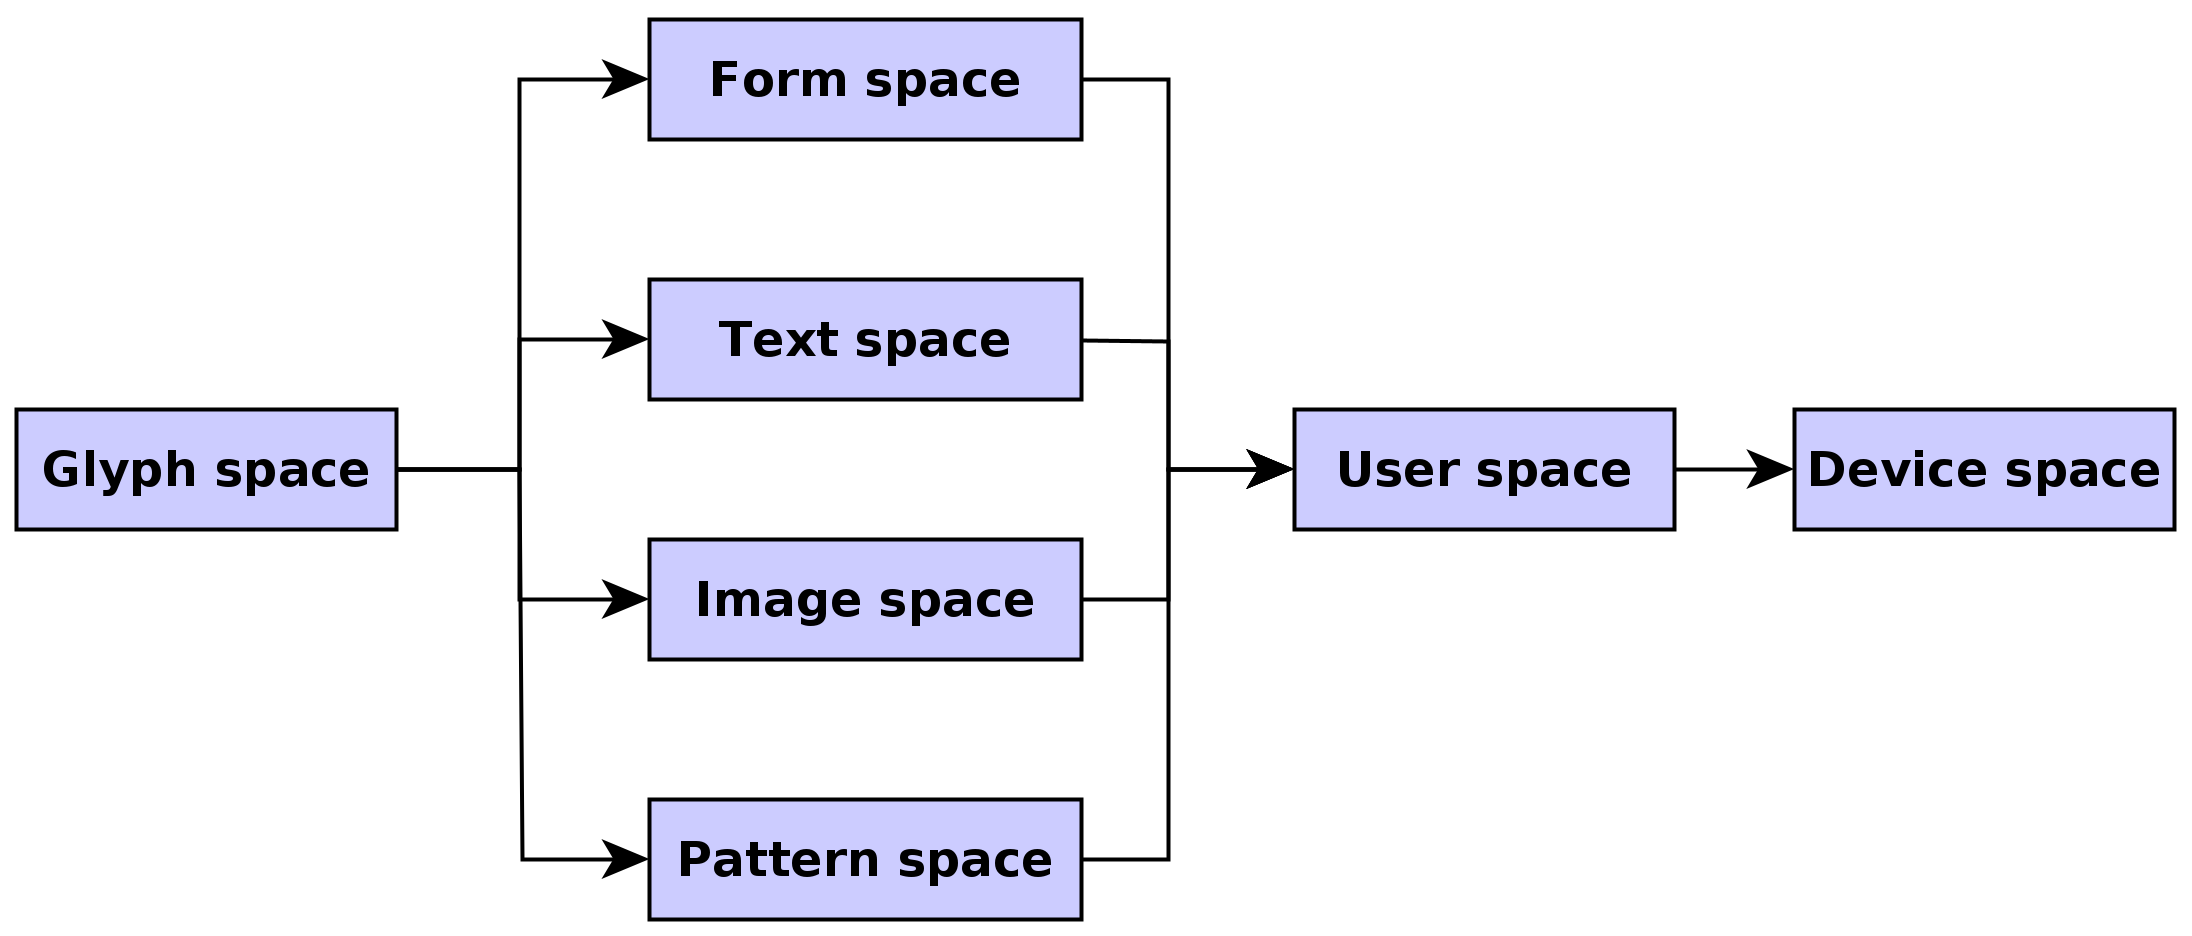
\includegraphics[width=11cm]{imaxes/espacios-coordenadas.png}
\end{figure}

¿Por qué el formato PDF almacena las coordenadas de las regiones?

\section{El formato HOCR}
\section{Herramientas y librerías}

\begin{itemize}
	\item Extracción de texto: Apache PDFBox, pdftotext
	\item OCR: Tesseract
	\item Pretty print de JSON: jq
\end{itemize}

%%%%             %%%%
%%%% METODOLOGÍA %%%%
%%%%             %%%%

\chapter{Metodología}
\label{chap:metodologia}

\section{Planificación económica}

La metodología utilizada para el desarrollo del proyecto es una metodología Scrum adaptada a las particularidades del proyecto. Una vez seleccionadas las herramientas de trabajo y llevada a cabo una primera versión del \emph{engine}, el desarrollo de cada modelo siguió un proceso iterativo. En términos de sprints serían los siguientes:

\lettrine{E}{l} comienzo de este proyecto consistió en una amplia búsqueda de aproximaciones y herramientas que orientasen la construcción del producto final.

También se hacía necesario decidir que tareas se considerarían como responsabilidad del software y cuales no. Se trataba de acotar el problema para obtener unos resultados satisfactorios. 

\section{Sprint a}

La primera de las tareas a abordar en el trabajo fue investigar la viabilidad del proyecto. Planteado el problema, no se conocía una solución directa. El resultado de esta primera fase de investigación fue conocer la existencia de los formatos para descripción del contenido del documentos digitalizados.

\begin{itemize}
    \item Investigación de qué herramientas utilizar en Linux para tratar con ficheros PDF.
    \item Información del formato HOCR
    \item Información sobre el formato PDF
    \item Uso de Tesseract
\end{itemize}

\section{Sprint b - Preparación del engine}
\begin{itemize}
    \item Estructura de directorios
    \item Creación del Makefile
    \item Creación de los scripts
    \begin{itemize}
        \item Generación único para cada petición
        \item Recepción de los ficheros
        \item Renombrado de los fichero para tratamiento seguro
        \item Discriminación de ficheros basados en texto y basados en imagen
        \item Extracción de texto con pdftotext
        \item Invocación de las aplicaciones para generar el lenguaje intermedio y el lenguaje estructurado
    \end{itemize}
\end{itemize}

\section{Primer modelo}
\section{Segundo modelo}
\section{Tercer modelo}
\section{Modelo n...}
\section{Sprint f - Adaptaciones para la interfaz gráfica}
\begin{itemize}
    \item \emph{Dockerizacion}
    \item Generación de imágenes para cada página de los PDF basados en texto
    \item Poblar el directorio de salida con los resultados
\end{itemize}

\section{Resultados de la planificación}

Aquí debe explicarse los desvíos en la planificación tanto temporales como económicos.

%%%%                       %%%%
%%%% ENTORNO DE DESARROLLO %%%%
%%%%                       %%%%

\chapter{Entorno de desarrollo}
\label{chap:entorno-desarrollo}

\lettrine{E}{l} entorno de desarrollo utilizado consistió en una distribución Ubuntu GNU/Linux con versiones actualizadas de las aplicaciones utilizadas en el proyecto. Para el desarrollo en lenguaje Python se optó por el IDE Eclipse con el plugin Pydev, específico para desarrollo con lenguaje Python. El codigo C y los scripts Bash fueron realizados con el editor Atom.

%%%%            %%%%
%%%% MATERIALES %%%%
%%%%            %%%%
\chapter{Materiales}
\label{chap:materiales}

Análisis de los documentos utilizados para el desarrollo del proyecto. Modelos PDF de texto facilitados por Betmedia. Modelos PDF imagen facilitados por Solco.

Caracterización de las regiones de interés.

Datos para identificar los documentos. En este caso, NIF, CIF.

 %%%%                %%%%
%%%% IMPLEMENTACIÓN %%%%
%%%%                %%%%

\chapter{Implementación}
\label{chap:implemetación}

La implementación está diseñada para recibir peticiones de conversión y generar la salida correspondiente en formato estructurado. El número de ficheros que se pueden tratar en cada ejecución solo está limitado por las capacidades del sistema operativo donde se ejecute. Cada invocación crea una tarea en el sistema, que se gestiona de forma individual. Una vez que se reciben los ficheros para su tratamiento, se produce una ruta específica para ese trabajo y comienza el proceso. En cada etapa se crean nuevos ficheros intermedios que, según se verá más adelante, se mueven a destinos designados para cada paso. El motor encargado de conducir el flujo de información está implementado en lenguaje Bash. El \emph{engine} utiliza varias herramientas complementarias, disponibles en cualquier distribución Linux. Se complementan con el generador de código intermedio y los parsers para cada modelo de documento.

Existen, por tanto, tres partes que se detallarán en las siguientes páginas:

\begin{itemize}
    \item Un motor o \emph{engine} creado con \emph{scripts} en lenguaje Bash. Su cometido es recepcionar los ficheros y transformarlos paso a paso hasta la obtención de la salida final.
    \item Una aplicación Python encargada de generar el lenguaje intermedio que va a ser procesado.
    \item Una familia de escáners y parsers desarrollados empleando Flex \cite{estes_flex_2021} y GNU Bison \cite{free_software_foundation_inc_bison_nodate}. Toman como entrada el lenguaje intermedio y lo traducen a un formato estructurado.
\end{itemize}

Se describen a continuación cada una de ellas.

\section{El engine}
La herramienta se planteó como un software que pudiera ser capaz de recibir uno o varios ficheros en cada invocación. Una vez recibido, cada input debía ser clasificado e identificado para su correcto tratamiento. Dado que la entrada y la salida serían ficheros, resultaba natural utilizar un lenguaje de programación con facilidades para la manipulación de ficheros. Por ser el entorno de operación y desarrollo un sistema GNU/Linux, se optó por emplear el intérprete de \emph{shell} Bash.

Por tratarse de un conjunto de \emph{scripts}, este \emph{pipeline} es flexible tanto para añadir nuevos pasos como para quitarlos. La razón para hacerlo de este modo radica en posibilitar la incorporación de nuevas técnicas de procesado de cualquiera de los aspectos, como el tratamiento de imagen o extracción de texto. Cada \emph{script} es independiente y puede ser ser activado o desactivado.

%% Convenio de nombrado para evitar perder información o mezclar páginas

%% Elaboración de las plantillas: Las plantillas son ficheros en formato JSON. Contienen las coordenadas de la geometría para las regiones de interés.

%% Generación del lenguaje intermedio: el sistema de generación de lenguaje intermedio debía ser necesariamente flexible. Para poder aplicar técnicas distintas. Se optó por utilizar Python, que tiene mucho soporte y una gran colección de librerías disponibles.

%% Detección de subregiones: Se diseñó un algoritmo sencillo pero eficaz para decidir si una región era subregión de otra dada.

%% Aproximación para la identificación de las lineas individuales: Esta aproximación se basó en intentar caracterizar las lineas mediante propiedades sencillas. La aproximación no dio resultado.

%% Mejora de tiempos: Inicialmente se utilizada el tipo de dato Set y sus operaciones para comprobar la inclusión de unas regiones en otras. Esta aproximación, aunque funcional, no resultaba rápida para su ejecución durante el desarrollo. Se realizó una mejora que comprueba las propiedades geométricas en lugar de basarse en lógica de conjuntos.

%% Obtención de información estructurada
%%%% Flex
%%%% Bison

%% Despliegue de la aplicación

%% Cambios para integrarse con la GUI
%%%% Exponiendo las coordenadas 
%%%% Uso de Docker

\section{Estructura física}

Para entender más fácilmente las características de la implementación se describen primero la estructura de directorios que conforman el proyecto. La aplicación se compila y distribuye por medio de un \verb|Makefile|. También se implementó un fichero \verb|Dockerfile|  configurado para generar la correspondiente imagen Docker del programa. 
La estructura y funcionalidad de los directorios del proyecto es importante para detallar como se trata la entrada. Esta estructura general se puede consultar gráficamente en XXX. Los principales directorios utilizados son:

\begin{itemize}
    \item \verb|conf|, empleado para las configuraciones del \emph{engine}, también la configuración de Tesseract y los datos de entrenamiento.
    \item \verb|data| contiene información de los modelos soportados. Principalmente los identificadores utilizados para reconocer los documentos y las plantillas que relacionan las regiones seleccionadas.
    \item \verb|doc| está dedicado a la documentación del proyecto y a esta memoria, escrita en formato \LaTeX. También contiene todos los ejemplos de ficheros PDF utilizados.
    \item \verb|engine| tiene como finalidad alojar todos los \emph{scripts} del \emph{engine}.
    \item \verb|input| no está en el repositorio, sino que se crea bajo demanda, es la ruta base para la entrada de datos utiliza por la aplicación. El nombre se escoge en la configuración del \emph{engine}.
    \item \verb|script| mantiene varios \emph{scripts} auxiliares utilizados principalmente para facilitar las ejecuciones durante el desarrollo.
    \item \verb|tool-gen-language| es la carpeta dedicada a los fuentes de la herramienta de generación de lenguaje intermedio.
    \item Por último, \verb|tool-parser| contiene la aplicación Flex/Bison y los \verb|plugins| que convierten el lenguaje intermedio a la salida JSON.
\end{itemize}

\section{Tratamiento inicial de la entrada}

La herramienta es un software \verb|backend|, no está pensada para que un usuario realice las ejecuciones de la aplicación manualmente. Por ello, y aunque no se desarrolló un API para acompañar la solución, si que se definieron varias características con la finalidad de facilitar la depuración durante el desarrollo y servir de primera aproximación para una futura integración en un sistema con un diseño por capas.

Cada ejecución se lleva a cabo en un directorio propio donde se almacena la entrada, se realiza el tratamiento y se ubicar la salida. Además se facilita al programa llamante un identificador que este debe utilizar para la recuperación de los resultados. La ruta al directorio que contiene todas las carpetas de todas las ejecuciones el es directorio \verb|input| mencionado anteriormente.

Para evitar colisiones en las rutas de trabajo entre distintas ejecuciones se obtiene una marca de tiempo del instante de recepción de la petición. Para obtener este \emph{timestamp} se utiliza el comando \verb|date| de la forma siguiente:

\begin{verbatim}
diego@CompaqCQ57:galiasdoc$ date -u +"%s%6N"
1616623143141490
diego@CompaqCQ57:galiasdoc$
\end{verbatim}

A continuación se presenta la secuencia de pasos que conforman en comienzo de una tarea en el sistema. La primera acción ocurre cuando el invocador del sistema ejecuta el \emph{script} \verb|get-job-id.sh|. Este crea el nuevo directorio para el trabajo y todos los directorios internos. Se devuelve el identificador de trabajo al llamador.

En este momento el llamador debe copiar el fichero de entrada en la ruta \verb|job_id/frontend|. Por último se inicia la ejecución cuando se llama al \emph{script} \verb|run.sh|. La entrada que habrá de tratar se indica con el \verb|job_id| pasado como parámetro. Los pasos se pueden seguir visualmente en la figura \ref{fig:inicio-aplicacion}.

A partir de este momento el sistema comienza a trabajar. Cada acción llevada a cabo se indica con un mensaje por la salida estándar de la consola. Cuando finaliza se notifica con una marca de tiempo del momento final en la ruta \verb|input/job_id/done-<timestamp>|.

\begin{figure}[hp!]
  \centering
  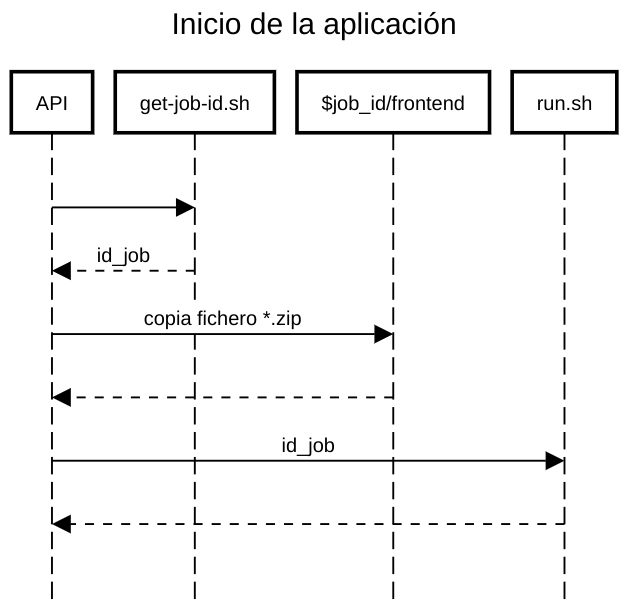
\includegraphics[width=11cm]{imaxes/inicio-aplicacion.png}
  \caption{Secuencia de inicio de la aplicación}
  \label{fig:inicio-aplicacion}
\end{figure}

%% Cambiar diagrama con flecha saliente para indicar que se ejecutan los pasos del engine
%% Cambiar "copia fichero *.zip" por "datos entrada"
%% La linea de finalización debe devolver el evento de finalización

\section{Flujo del engine}

Cuando se invoca el \emph{script} \verb|run.sh| se realizan en secuencia todos los pasos que acaban generado la salida en formato estructurado.

\begin{enumerate}
    \item Descompresión de la entrada.
    \item Renombrado seguro de los ficheros.
    \item Extracción de texto con \emph{pdftotext}.
    \item Clasificación de los casos basados en texto y aquellos basados en imagen.
    \item Generación de imágenes para los documentos basados en texto.
    \item Aplicación del OCR para los casos basados en imagen.
    \item Identificación de cada documento.
    \item Generación del lenguaje intermedio.
    \item Invocación del parser necesario.
    \item Publicación de los resultados en el directorio de salida.
\end{enumerate}

\section{Generación del lenguaje intermedio}
\section{Salida en lenguaje estructurado}
 %%%%              %%%%
%%%% CONCLUSIONES %%%%
%%%%              %%%%

\chapter{Conclusiones}
\label{chap:conclusiones}

Decidir en qué fase realizar un tratamiento determinado no es siempre trivial.

Los documentos deben ser tratados individualmente. Cada PDF no debe contener páginas mezcladas. Separar páginas de distintos documentos es otro problema en si mismo.

Para un correcto procesamiento los documentos que se proporcionen al sistema deben ser digitalizados 

\section{Limitaciones de la solución}
La resolución seleccionada para las imágenes tiene gran implicación en varios aspectos.
\begin{itemize}
    \item Las plantillas solo representan una resolución determinada
    \item Imposibilidad de distinguir lineas distintas en las tablas
\end{itemize}

\section{Requisitos para un correcto reconocimiento del texto}
Digitalización automática de los documentos

%%%%                %%%%
%%%% TRABAJO FUTURO %%%%
%%%%                %%%%

\section{Trabajo futuro}

\begin{itemize}
    \item Generación de coordenadas homogéneas para los casos procedentes de imagen y los procedentes de texto.
    \item Construcción de un asistente para generar las plantillas. Seleccionar el tipo de región y coordenadas de forma visual.
    \item Implementar un sistema para la notificación asíncrona a la finalización de los trabajos.
    \item incorporación de una base de datos no relacionar para el almacenamiento de las plantillas.
\end{itemize}


 %\chapter{Conclusións}
\label{chap:conclusions}

\lettrine{D}{erradeiro} capítulo da memoria, onde se presentará a
situación final do traballo, as leccións aprendidas, a relación coas
competencias da titulación en xeral e a mención en particular,
posibles liñas futuras,\dots

\Blindtext


 %%%%%%%%%%%%%%%%%%%%%%%%%%%%%%%%%%%%%%%%
 % Apéndices, glosarios e bibliografía  %
 %%%%%%%%%%%%%%%%%%%%%%%%%%%%%%%%%%%%%%%%

 \appendix
 \appendixpage
 %%%%           %%%%
%%%% ADICIONAL %%%%
%%%%           %%%%

\chapter{Material adicional}
\label{chap:adicional}

% TODO añadir imágenes de los documentos tratados

% TODO Manual de la herramienta

% TODO valorar si añadir capturas de 
% TODO - formato de un PDF

\lettrine{A}{unque}
 \chapter{Fuentes de información propias}
\label{chap:preparación}

A la hora de ponerse a escribir la memoria, es útil disponer de registros o un histórico con todo aquello ocurrido e importante.

En este caso se dispuso de varias fuentes de información a las que recurrir:

\begin{itemize}
    \item Mensajes de correo electrónico intercambiados con el director y otras personas implicadas en el proyecto.
    \item Cuadernos manuscritos. Contienen notas elaboradas durante los momentos de trabajo y reuniones.
    \item Las conversaciones en formato chat mantenidas con Arturo Silvelo por medio de Teams, la herramienta que la UDC pone a disposición de los miembros de la Universidad.
\end{itemize}

Toda esta información de apoyo es útil al menos desde dos puntos de vista. Aquellos relacionados con los tiempos del proyecto: señalización de hechos importantes o hitos alcanzados. Y problemas resueltos. Esto es debido a que el registro de las dificultades acontecidas y el diseño de algoritmos particulares se hizo la mayor parte de las veces, en papel.

\section{Fechas relevantes}

Primera fase de desarrollo con los datos de Solco

\begin{center}
\begin{tabular}{ |c|c| } 
 04-10-2019 & Primera muestra de ficheros \\
 29-10-2019 & Primera reunión con los clientes \\
 03-12-2019 & Ángel crea el repositorio SVN \\
 03-02-2020 & Me doy cuenta de que no se espera se vaya a aplicar un modelo de aprendizaje \\
 06-02-2020 & 2º demostración en showroom del CITIC \\
\end{tabular}
\end{center}  

Comienzo del teletrabajo

\begin{center}
\begin{tabular}{ |c|c| }  
 08-01-2020 & Primera referencia a la estructura de directorios. \\
 13-01-2020 & Reunión de seguimiento con Victor, Dafonte. \\
 13-03-2020 & Cierra el CITIC por el Covid y nos envían para casa. \\
 02-04-2020 & Primer día en Odeene (jueves). \\
 14-04-2020 & Antonio Rojo facilita facturas Citic. \\
 14-04-2020 & Llegan las facturas de Betmedia. \\
 15-04-2020 & Planteamiento del nuevo modelo con los doc OVH. \\
 20-04-2020 & Firma del anteproyecto. \\
 21-04-2020 & Cambio al modelo de parsers como \emph{plugins}. \\
 28-04-2020 & Decisión de entrada separada por documento. \\
 27-04-2020 & Último commit en SVN. \\
\end{tabular}
\end{center} 

Segunda fase de desarrollo.

\begin{center}
\begin{tabular}{ |c|c| }  
 22-06-2020 & Primer commit del verano en git \\
 29-07-2020 & Primera reunión con Arturo \\
 12-08-2020 & Reunión con Arturo – confusión px vs. cm. \\
 17-08-2020 & Comienzo vacaciones Odeene \\
 19-08-2020 & Detectar que una linea ocupa varias columnas \\
 25-08-2020 & La aplicación funciona con Docker \\
 26-08-2020 & Petición cambios adaptación UI: directorio de salida único, imágenes de los PDF \\
 26-08-2020 & Cambio del jobId: fecha → timeStamp \\
 02-09-2020 & Las words llevan el nº de página \verb|p1w10| \\
 04-09-2020 & Fin vacaciones Odeene \\
 15-11-2020 & Último commit de esta fase
\end{tabular}
\end{center}

Más fechas por localizar
\begin{itemize}
    \item ¿Cuándo se me comunica que perdimos al primer cliente?
\end{itemize}

\begin{center}
    \begin{tabular}{c|c|c}
     25-11-2019 & 04-12-2019 & Primer repositorio Git \\
     03-12-2019 & 09-01-2020 & Segundo repositorio Git \\
     03-12-2019 & 27-04-2020 & Repositorio SVN \\
     22-06-2020 & 15-11-2020 & Último repositorio Git
    \end{tabular}
\end{center}

\section{Ideas importantes}

En la primera etapa de desarrollo había previsto crear unos \emph{tipos} de datos en la fase de generación del lenguaje intermedio. Estos tipos serían tratados luego por Flex y Bison. En la generación del lenguaje intermedio se identificaban las fechas, los números, y lo strings.

Aunque en el apartado de \ref{chap:implemetación} se explica el trabajo desde un punto de vista secuencial, lo cierto es que una vez seleccionadas las herramientas de trabajo y escrito en \emph{engine}, el resto de desarrollo es circular para cada uno de los nuevos modelos que hay que incorporar.

La \textbf{transformada de Hough} es un algoritmo que facilitó localizar lineas en dos de los modelos de documentos. Sin él no 

\underline{lunes, 13/01/2020}

Trabajos probablemente dirigidos por Dafonte:

\begin{itemize}
    \item TFG-INF 375
    \item TFG-INF 426
    \item TFG-INF 457
\end{itemize}

\underline{lunes, 20/01/2020}

Ejemplo de los tres tipos de lineas que hay en uno de los documentos:

\begin{itemize}
    \item Líneas de la factura
    \item Descripción de la agrupación por albarán
    \item Totales
\end{itemize}

Esta información, aunque fácil de distinguir para las personas, mucho más difícil de modelar.

\underline{lunes, 3/02/2020}

Inicialmente pensaba construir un único parser para todos los documentos. Al identificar cada documento sería fácil, tratarlo de forma individual. Nada más lejos de la realidad. Las colisiones en la gramática serían imposibles de resolver. Además con el enfoque final, se consigue un modelo comercial más adecuado: cada comprador de la aplicación recibe únicamente los parsers a los que tiene derecho.

Un fichero PDF es texto en formato ASCII de 7 bits. Todos los documentos contienen una cabecera que indica la versión del formato: \verb|%PDF1.7|.

\underline{lunes, 23/03/2020}

Mejora del tiempo utilizado para decidir si una word está dentro de una región de interés o no. La implementación inicial se basaba en el tipo Set. La nueva implementación tiene en cuenta las posiciones de la geometría de la palabra y la región.

\underline{(Probablemente) sabado, 11/07/2020:}

Flujo para el tratamiento de la información:

\begin{figure}[hp!]
  \centering
  \includegraphics[width=9cm]{imaxes/h-implementacion/flujo-información.png}
\end{figure}

Idea de un requisito: se desea mostrar los errores detectados, aunque no definen cuales errores. Pero cuidado, en esta herramienta no está incluido el frontend.

\underline{lunes, 13/07/20}

Idea de diseño: guardar los datos siempre en listas y procesar las listas. La ventaja es que si es una lista vacía no habrá salida, pero no hay que preocuparse sobre la existencia de los datos, como comprobaciones para evitar null pointers.

Un problema encontrado: una misma linea puede tener palabras a distintas alturas. Esto lleva a recordar que en el contexto de este desarrollo hay dos cosas distintas que se entienden por lineas. La primera es la idea natural de lo que es una linea para una persona que lee el documento. La segunda se refiere a la secuencia de palabras que conforman parte o la totalidad de la linea natural. Esto es así porque los contenidos de una linea natural pueden quedar separados en la extracción del texto. Puede haber otros contenidos intermedios. Esto ocurría por ejemplo con las facturas donde se listaban grupos de facturas. La siguiente situación donde puede ocurrir esto es debida a las columnas que trocean las lineas.

Sobre las regiones. Existen regiones cuyos contenidos podrían asimilarse a matrices. En particular 

\begin{math}
\begin{pmatrix}
  a_1 & a_2 & a_3 & a_4 \\
  b_1 & b_2 & b_3 & b_4 \\
  c_1 & c_2 & c_3 & c_4
\end{pmatrix}
\end{math}

La pregunta subyacente es, ¿puedo tratar del mismo modo los datos horizontales y verticales?

\underline{jueves, 23/07/2020}

Sobre los documentos multipágina:
\begin{itemize}
    \item Al mismo tiempo que se extrae el texto, se puede asociar el número de página.
    \item Luego se puede pasar el número como un parámetro.
    \item Si dos páginas son iguales, este conocimiento se define en Flex. Cuando se trata el tocket de la página $P_2$, sabiendo que es igual a la página $P_1$, se devuelve a Bison la $P_1$.
\end{itemize}

\underline{martes, 28/07/20}

Tecnologías para hacer un API intermedio entre la herramienta y el frontend. Pedro Lorenzo dio la idea de utilizar Node.js. Aunque finalmente se optó por no incluir ningún API entre el \emph{backend} y el \emph{frontend}.

\underline{miércoles, 29/07/2020}

Nombres de las empresas que facilitaron sus documentos para la elaboración de la herramienta:
\begin{itemize}
    \item Solco
    \item Betmedia
    \item Citic
\end{itemize}

\underline{sábado, 8/08/2020}

Se comparan las salidas XML y HOCR para una misma región simple y pequeña. No coinciden el orden de los elementos de salida.

 \printglossary[type=\acronymtype,title=\nomeglosarioacronimos]
 \printglossary[title=\nomeglosariotermos]

 \bibliographystyle{IEEEtranN}
 \bibliography{\bibconfig,bibliografia/bibliografia}
 \cleardoublepage
 
\end{document}

%%%%%%%%%%%%%%%%%%%%%%%%%%%%%%%%%%%%%%%%%%%%%%%%%%%%%%%%%%%%%%%%%%%%%%%%%%%%%%%%
